
% xetex expected
\documentclass[xetex,professionalfont]{beamer}

% we want math
\usepackage{amsmath}

% fixes and extensions to amsmath
\usepackage{mathtools}

% additional math symbols
\usepackage{amssymb}

% good-looking fractions in text via \sfrac
\usepackage{xfrac}

% fix spaces after custom commands (see below for examples)
\usepackage{xspace}

% minted allows for fancy syntax highlighting (requires python with pygments)
% usage:
%   \begin{minted}{python}
%   codeb
%   \end{minted}
\usepackage{minted}

% better looking tables
% usage:
%   begin with a \toprule, write a single row of column headings,
%   then add \midrule and after the columns of data we finish with \bottomrule
% example:
%   \begin{tabular}{llr} \toprule
%   Animal & Description & Price \midrule
%   cat & foo & 10 \\
%   dog & bar & 20 \\ \bottomrule
%   \end{tabular}
% note that good tables generally neither have vertical rules nor double rules
\usepackage{booktabs}

% system font support (requires xetex or luatex)
\usepackage{fontspec}
\setmonofont[Scale=0.7]{Cousine} % part of ttf-chromeos fonts on Arch

% improve microtypography
\usepackage{microtype}

% multi-language quotes for babel
\usepackage{csquotes}

% easy way to include copyright information
\usepackage{copyrightbox}

% better bibliographies
\usepackage[backend=biber,style=numeric]{biblatex}

% language support (english,ngerman)
\usepackage[english]{babel}

% -----------------------------------------------------------------------------

% copyright font style
\makeatletter\renewcommand{\CRB@setcopyrightfont}{\tiny\color{lightgray}}

% make emph bold
\DeclareTextFontCommand{\emph}{\bfseries}

% use proper fonts for math
% \usefonttheme[onlymath]{serif}

% use tuwcvl beamer theme
\usetheme{tuwcvl}

% add bib file
\addbibresource{literature.bib}

% smileys :)
\newfontfamily\DejaSans{DejaVu Sans}

% -----------------------------------------------------------------------------

% common english abbreviations
\newcommand{\ie}{\mbox{i.e.}\xspace} % i.e.
\newcommand{\eg}{\mbox{e.g.}\xspace} % e.g.

% math - argmin and argmax
\DeclareMathOperator*{\argmin}{arg\,min}
\DeclareMathOperator*{\argmax}{arg\,max}

% shortcuts for number ranges
\newcommand{\NN}{\mathbb{N}}
\newcommand{\ZZ}{\mathbb{Z}}
\newcommand{\QQ}{\mathbb{Q}}
\newcommand{\RR}{\mathbb{R}}

% bold vectors
\renewcommand{\vec}[1]{\ensuremath{\mathbf{#1}}}

% vector shortcuts
\newcommand{\va}{\vec{a}}
\newcommand{\vb}{\vec{b}}
\newcommand{\vc}{\vec{c}}
\newcommand{\ve}{\vec{e}}
\newcommand{\vr}{\vec{r}}
\newcommand{\vs}{\vec{s}}
\newcommand{\vt}{\vec{t}}
\newcommand{\vu}{\vec{u}}
\newcommand{\vv}{\vec{v}}
\newcommand{\vw}{\vec{w}}
\newcommand{\vx}{\vec{x}}
\newcommand{\vy}{\vec{y}}
\newcommand{\vz}{\vec{z}}

% -----------------------------------------------------------------------------

\title{Computer Vision Systems Programming VO}
\subtitle{Programming Languages and Libraries}
\author{Christopher Pramerdorfer}
\institute{Computer Vision Lab, Vienna University of Technology}

\begin{document}

% -----------------------------------------------------------------------------

\begin{frame}
\maketitle
\end{frame}

% -----------------------------------------------------------------------------

\begin{frame}
\frametitle{Topics}

Characteristics of Computer Vision (CV) programming
\begin{itemize}
	\item Implications on language choice
\end{itemize}

\bigskip
Which language is the best? {\DejaSans 😇}

\bigskip
Overview of popular languages and libraries
\begin{itemize}
	\item Matlab
	\item Python
	\item C++
\end{itemize}

\bigskip
Suggestions on language selection

\end{frame}

% -----------------------------------------------------------------------------

\begin{frame}
\frametitle{Characteristics of CV Programming}
\framesubtitle{Image Processing}

We often start with Image Processing (IP)
\begin{itemize}
	\item Resampling, normalization, color conversion
	\item Feature extraction
\end{itemize}

\medskip
Involves operations on arrays / matrices

\bigskip
Many IP operations are local and sequential
\begin{itemize}
	\item Favors languages with fast random access to pixels % don't code loops in matlab should sound familiar
\end{itemize}

\end{frame}

% -----------------------------------------------------------------------------

\begin{frame}
\frametitle{Characteristics of CV Programming}
\framesubtitle{Many IP Operations are Local and Sequential}

Resampling is independent for each pixel\\
Usually involves some form of interpolation

\bigskip
\begin{center}
	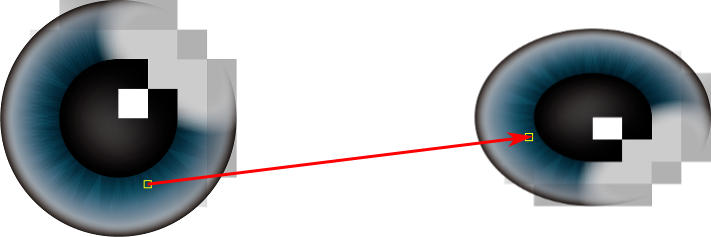
\includegraphics[width=8cm]{figures/resampling.png}
\end{center}

\end{frame}

% -----------------------------------------------------------------------------

\begin{frame}
\frametitle{Characteristics of CV Programming}
\framesubtitle{Many IP Operations are Local and Sequential}

Local neighborhood operators such as linear filtering:
\[
 f'(x,y)=\sum_{i,j}f(x+i,y+j)\,h(i,j)
\]

\medskip
\begin{center}
	\copyrightbox[b]
	{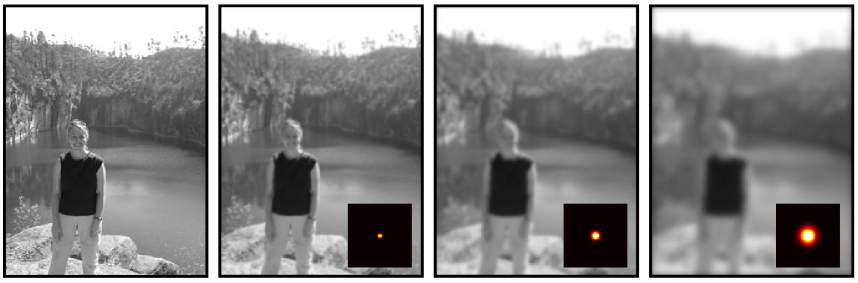
\includegraphics[width=8cm]{figures/blur-example.png}}
	{\centering Image from \cite{prince12}}
\end{center}

\end{frame}

% -----------------------------------------------------------------------------

\begin{frame}
\frametitle{Characteristics of CV Programming}
\framesubtitle{Numerical Computing}

More generally, CV programming is all about numbers

\bigskip
Often, there are many of them:
\begin{itemize}
	\item BD stream: $\sim$ 50 million/sec % 1920*1080*24
	\item Large optimization problems (\eg bundle adjustment) \\ \url{https://www.youtube.com/watch?v=HrgHFDPJHXo}
\end{itemize}

\bigskip
Some languages are better at crunching numbers than others
\begin{itemize}
	\item Faster, more memory-efficient
\end{itemize}

\end{frame}

% -----------------------------------------------------------------------------

\begin{frame}
\frametitle{Characteristics of CV Programming}
\framesubtitle{Does efficiency matter?}

But does efficiency matter?
\begin{itemize}
	\item Researchers often don't care
	\item Companies usually do % run more analysis channels on a the same machine = money saved
	\item Sometimes there are hard constraints (cars, space missions)
\end{itemize}

\medskip
\begin{center}
	\copyrightbox[b]
	{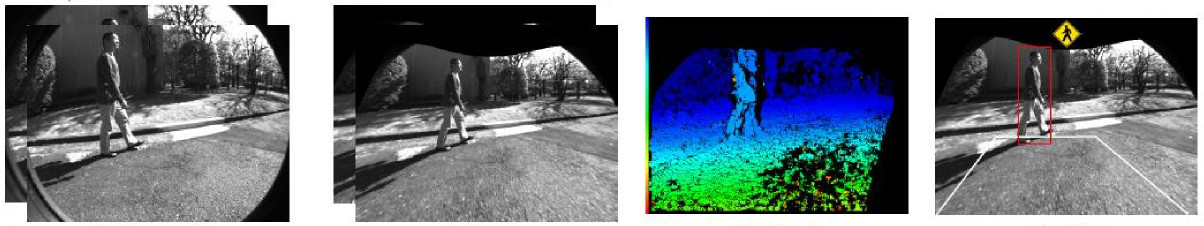
\includegraphics[width=10cm]{figures/car-pedestrian.jpg}}
	{\centering Image by Ryuzo Okada, Toshiba}
\end{center}

\end{frame}

% -----------------------------------------------------------------------------

\begin{frame}
\frametitle{Characteristics of CV Programming}
\framesubtitle{Does efficiency matter?}

\emph{It depends}

\bigskip
Design choices can have a bigger impact than language
\begin{itemize}
	\item Use appropriate data structures
	\item Utilize multiple CPU cores, GPUs
\end{itemize}

\bigskip
Language bottlenecks can be avoided by switching language
\begin{itemize}
	\item Implement parts in C, call from Matlab, Python
\end{itemize}

\end{frame}

% -----------------------------------------------------------------------------

\begin{frame}
\frametitle{Choosing a Programming Language}

In summary, efficiency is often of little concern

\bigskip
There are other factors:
\begin{itemize}
	\item Ease of development (language features, libraries, IDEs)
	\item OS and platform support % does it run on all OS? does it run on ARM like the odroid shown below?
	\item License fees % matlab is 2000 euros as of oct 2014
\end{itemize}

\begin{center}
	\copyrightbox[b]
	{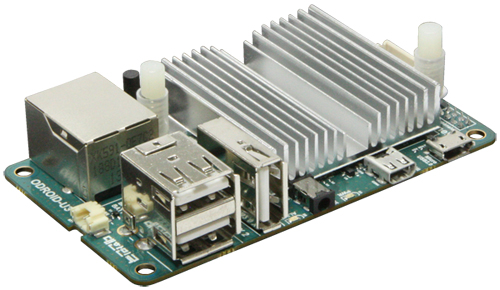
\includegraphics[width=4cm]{figures/odroid-u3.jpg}}
	{\centering Image from \url{pixhawk.org}}
\end{center}

\end{frame}

% -----------------------------------------------------------------------------

\begin{frame}
\frametitle{Choosing a Programming Language}

\emph{There is no \enquote{best} language}, it depends:
\begin{itemize}
	\item On the task at hand % pedestrian detection ...
	\item On the operating conditions % for a paper? speed usually not important / for use in cars? different story!
\end{itemize}

\bigskip
Let's take a look at some popular languages and libraries ...

\end{frame}

% -----------------------------------------------------------------------------

\begin{frame}
\frametitle{Popular CV Programming Languages}

\begin{figure}
\centering
{\copyrightbox[b]
	{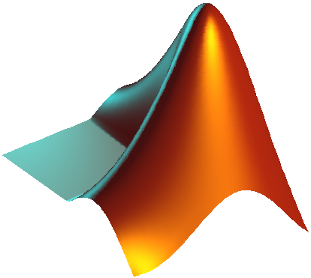
\includegraphics[width=2.8cm]{figures/matlab-logo.png}}
	{\centering Image from \url{matworks.de}}}\quad
{\copyrightbox[b]
	{
\includegraphics[width=4.5cm]{figures/python-logo.png}}
	{\centering Image from \url{python.org}}}\quad
{\copyrightbox[b]
	{
\includegraphics[width=2.2cm]{figures/cpp-logo.jpg}}
	{\centering Image from \url{cplusplus.se}}}
\end{figure}

\end{frame}

% -----------------------------------------------------------------------------

\begin{frame}
\frametitle{Popular CV Programming Languages}
\framesubtitle{Matlab}

\begin{columns}
\column{0.65\textwidth}

Numerical computing environment \\
Commercial software (student licenses)

\bigskip
Widely used in academics \\
Used in many courses at TU Wien
\begin{itemize}
	\item You probably already know it
\end{itemize}

\column{0.25\textwidth}

\begin{center}
{\copyrightbox[b]
	{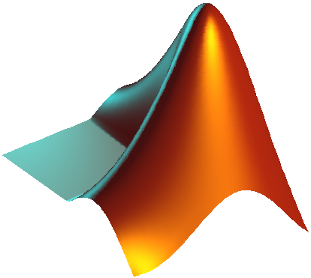
\includegraphics[width=2.3cm]{figures/matlab-logo.png}}
	{\centering Image from \url{matworks.de}}}
\end{center}

\end{columns}

\end{frame}

% -----------------------------------------------------------------------------

\begin{frame}
\frametitle{Popular CV Programming Languages}
\framesubtitle{Matlab}

Pros:
\begin{itemize}
	\item Easy to learn and use
	\item Many high-quality toolboxes
\end{itemize}

\bigskip
Cons:
\begin{itemize}
	\item Not as fast/efficient from scratch as C++ % code is fast if vectorized, but that can be tedious work
	\item Commercial licenses are expensive
	\item Less suitable for general-purpose programming
\end{itemize}

\end{frame}

% -----------------------------------------------------------------------------

\begin{frame}
\frametitle{Popular CV Programming Languages}
\framesubtitle{Python}

\begin{columns}
\column{0.65\textwidth}

General-purpose programming language \\
Free and open source % This applies to the Cython reference implementation

\bigskip
No IP/CV functionality by default \\
But great open-source libraries:
\begin{itemize}
	\item NumPy
	\item SciPy, scikit-image % scipy is an umbrella term and contains all the below packages, but it is a library itself as well
	\item scikit-learn
	\item matplotlib
\end{itemize}

\column{0.25\textwidth}

\begin{center}
{\copyrightbox[b]
	{
\includegraphics[width=2.6cm]{figures/python-logo.png}}
	{\centering Image from \url{python.org}}}
\end{center}

\end{columns}

\end{frame}

% -----------------------------------------------------------------------------

\begin{frame}
\frametitle{Popular CV Programming Languages}
\framesubtitle{Python}

Pros:
\begin{itemize}
	\item Easy to learn and use
	\item Extensive standard library
	\item Free and open source
\end{itemize}

\bigskip
Cons:
\begin{itemize}
	\item Not as integrated as Matlab
	\item Not as fast/efficient from scratch as C++ % code is fast if vectorized, but that can be tedious work
\end{itemize}

\end{frame}

% -----------------------------------------------------------------------------

\begin{frame}
\frametitle{Popular CV Programming Languages}
\framesubtitle{Python -- NumPy}

\begin{columns}
\column{0.65\textwidth}

Fundamental numerical computing library

\bigskip
Arrays and matrices\\\medskip
Linear algebra\\\medskip
Matrix decompositions\\\medskip % svd, qr, cholesky
Fourier analysis

\column{0.25\textwidth}

\begin{center}
{\copyrightbox[b]
	{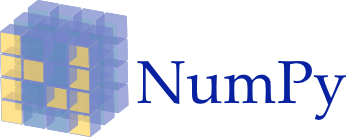
\includegraphics[width=2.6cm]{figures/numpy-logo.png}}
	{\centering Image from \url{github.com/numpy}}}
\end{center}

\end{columns}

\end{frame}

% -----------------------------------------------------------------------------

\begin{frame}
\frametitle{Popular CV Programming Languages}
\framesubtitle{Python -- SciPy}

\begin{columns}
\column{0.65\textwidth}

Family of scientific computing packages % like numpy, matplotlib

\bigskip
Optimization\\\medskip
Image processing\\\medskip % linear filtering, morphology, distance transform, segmentation
Statistics \& density estimation

\column{0.25\textwidth}

\begin{center}
{\copyrightbox[b]
	{
\includegraphics[width=2.3cm]{figures/scipy-logo.png}}
	{\centering Image from \url{scipy.org}}}
\end{center}

\end{columns}

\end{frame}

% -----------------------------------------------------------------------------

\begin{frame}
\frametitle{Popular CV Programming Languages}
\framesubtitle{Python -- scikit-image}

\begin{columns}
\column{0.65\textwidth}

Image processing library

\bigskip
Image transforms\\\medskip
Image filtering\\\medskip
Feature extraction\\\medskip
Segmentation % e.g. graphcut, watershed

\column{0.25\textwidth}

\begin{center}
{\copyrightbox[b]
	{
\includegraphics[width=2.6cm]{figures/ski-logo.png}}
	{\centering Image from \url{scikit-image.org}}}
\end{center}

\end{columns}

\end{frame}

% -----------------------------------------------------------------------------

\begin{frame}
\frametitle{Popular CV Programming Languages}
\framesubtitle{Python -- scikit-learn}

\begin{columns}
\column{0.65\textwidth}

Comprehensive machine learning library

\bigskip
Classification\\\medskip
Regression\\\medskip
Clustering\\\medskip
Dimensionality reduction

\column{0.25\textwidth}

\begin{center}
{\copyrightbox[b]
	{
\includegraphics[width=2.6cm]{figures/skl-logo.png}}
	{\centering Image from \url{goodfind.jp}}}
\end{center}

\end{columns}

\end{frame}

% -----------------------------------------------------------------------------

\begin{frame}
\frametitle{Popular CV Programming Languages}
\framesubtitle{Python -- matplotlib}

\begin{columns}
\column{0.65\textwidth}

Graph plotting library

\bigskip
Surface, wireframe, scatter, bar plots\\\medskip
Matlab-like syntax

\column{0.25\textwidth}

\begin{center}
{\copyrightbox[b]
	{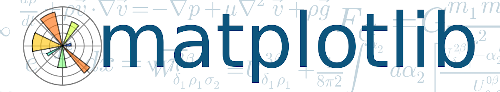
\includegraphics[width=2.6cm]{figures/matplotlib-logo.png}}
	{\centering Image from \url{matplotlib.org}}}
\end{center}

\end{columns}

\end{frame}

% -----------------------------------------------------------------------------

\begin{frame}
\frametitle{Popular CV Programming Languages}
\framesubtitle{C++}

\begin{columns}
\column{0.65\textwidth}

General-purpose programming language \\
Focus on performance and efficiency 

\bigskip
No IP/CV functionality by default \\
But great open-source libraries:
\begin{itemize}
	\item OpenCV
	\item Shark, Caffe
	\item MathGL
\end{itemize}

\column{0.25\textwidth}

\begin{center}
{\copyrightbox[b]
	{
\includegraphics[width=2.3cm]{figures/cpp-logo.jpg}}
	{\centering Image from \url{cplusplus.se}}}
\end{center}

\end{columns}

\end{frame}

% -----------------------------------------------------------------------------

\begin{frame}
\frametitle{Popular CV Programming Languages}
\framesubtitle{C++}

Pros:
\begin{itemize}
	\item Fast and memory-efficient
	\item Free and open source
\end{itemize}

\bigskip
Cons:
\begin{itemize}
	\item Harder to learn and master
	\item Slower and less convenient to code
\end{itemize}

\end{frame}

% -----------------------------------------------------------------------------

\begin{frame}
\frametitle{Popular CV Programming Languages}
\framesubtitle{C++ -- OpenCV}

\begin{columns}
\column{0.65\textwidth}

Comprehensive IP/CV library\\
Designed for real-time applications

\bigskip
Matrices and linear algebra\\\medskip
Image transforms and filtering\\\medskip
Feature extraction and matching\\\medskip
Stereo, structure from motion\\\medskip
Machine learning % boosting, trees, em, nn, svms, forests

\column{0.25\textwidth}

\begin{center}
{\copyrightbox[b]
	{
\includegraphics[width=2.3cm]{figures/opencv-logo.png}}
	{\centering Image from \url{opencv.org}}}
\end{center}

\end{columns}

\end{frame}

% -----------------------------------------------------------------------------

\begin{frame}
\frametitle{Popular CV Programming Languages}
\framesubtitle{C++ -- Shark, Caffe}

\begin{columns}
\column{0.65\textwidth}

Machine learning libraries

\bigskip
Optimization\\\medskip
Regression\\\medskip
Classification\\\medskip
Dimensionality reduction\\\medskip
Deep learning

\column{0.25\textwidth}

\begin{center}
{\copyrightbox[b]
	{
\includegraphics[width=2.3cm]{figures/shark-logo.png}}
	{\centering Image from \url{image.diku.dk}}}
\end{center}

\end{columns}

\end{frame}

% -----------------------------------------------------------------------------

\begin{frame}
\frametitle{Popular CV Programming Languages}
\framesubtitle{C++ -- MathGL}

\begin{columns}
\column{0.65\textwidth}

Graph plotting library

\bigskip
Surface, wireframe, scatter, bar plots

\column{0.25\textwidth}

\begin{center}
{\copyrightbox[b]
	{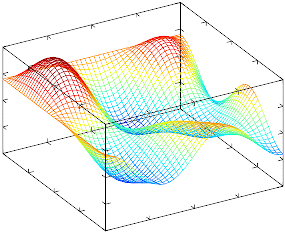
\includegraphics[width=2.6cm]{figures/mathgl-mesh.png}}
	{\centering Image from \url{mathgl.sourceforge.net}}}
\end{center}

\end{columns}

\end{frame}

% -----------------------------------------------------------------------------

\begin{frame}
\frametitle{Popular CV Programming Languages}
\framesubtitle{Remarks}

Comparable functionality
\begin{itemize}
	\item There are libraries for most CV tasks in all these languages
	\item This applies to other languages as well
\end{itemize}

\bigskip
Many libraries have language bindings
\begin{itemize}
	\item Python and Matlab bindings for OpenCV
\end{itemize}

\end{frame}

% -----------------------------------------------------------------------------

\begin{frame}
\frametitle{Language Comparison}

Task is to load, blur, show, and save an image

\end{frame}

% -----------------------------------------------------------------------------

\begin{frame}[fragile]
\frametitle{Language Comparison}
\framesubtitle{Matlab}

\begin{minted}{matlab}
img = imread('image.png'); % read
kernel = fspecial('gaussian', [5 5]); % blur
blur = imfilter(img, kernel); % blur
imshow(blur); % show
imwrite(blur, 'blur.png'); % save
\end{minted}

\end{frame}

% -----------------------------------------------------------------------------

\begin{frame}[fragile]
\frametitle{Language Comparison}
\framesubtitle{Python with scikit-image}

\begin{minted}{python}
img = skimage.io.imread('image.png') # read
blur = skimage.filter.gaussian_filter(img, sigma=1.7) # blur
skimage.io.imshow(blur) # show
skimage.io.show() # show
skimage.io.imsave('blur.png', blur) # save
\end{minted}

\end{frame}

% -----------------------------------------------------------------------------

\begin{frame}[fragile]
\frametitle{Language Comparison}
\framesubtitle{C++ with OpenCV}

\begin{minted}{cpp}
cv::Mat img = cv::imread("image.png"); // read
cv::Mat blur; // blur
cv::GaussianBlur(img, blur, cv::Size(5, 5), 0); // blur
cv::imshow("blur", blur); // show
cv::waitKey(0); // show
cv::imwrite("blur.png", blur); // save
\end{minted}

\end{frame}

% -----------------------------------------------------------------------------

\begin{frame}
\frametitle{Language Comparison}

Similar programming effort in the example case

\bigskip
For many larger CV tasks:
\begin{itemize}
	\item Matlab requires least effort
	\item Closely followed by Python
	\item No so closely followed by C++
\end{itemize}

\end{frame}

% -----------------------------------------------------------------------------

\begin{frame}
\frametitle{Language Comparison}

In summary, the discussed languages:
\begin{itemize}
	\item Differ in terms of execution speed and memory-efficiency
	\item Provide comparable CV programming functionality via libraries
	\item Differ in ease of development, licensing fees
\end{itemize}

\bigskip
So, to conclude:
\begin{itemize}
	\item \emph{There is no best CV language}
	\item \emph{Different tasks favor different languages}
\end{itemize}

\end{frame}

% -----------------------------------------------------------------------------

\begin{frame}
\frametitle{Suggestions on Language Selection}

Know the strengths and weaknesses of different languages\\\medskip
Be proficient in more than one language

\bigskip
Learn C++
\begin{itemize}
	\item Modern C++ is not a bad language if used correctly
	\item Many companies rely on it
\end{itemize}

\end{frame}

% -----------------------------------------------------------------------------

\begin{frame}
\frametitle{Bibliography}

\printbibliography

\end{frame}

\end{document}